\documentclass[nobib]{tufte-handout}

\newcommand{\bra}[1]{\left(#1\right)}
\usepackage{hyperref}
\usepackage[activate={true,nocompatibility},final,tracking=true,kerning=true,spacing=true,factor=1100,stretch=10,shrink=10]{microtype}
\usepackage{color}

% Set up the images/graphics package
\usepackage{graphicx}
\setkeys{Gin}{width=\linewidth,totalheight=\textheight,keepaspectratio}

\title{Notes for POL 23700 - Modern Weapons And International Relations}
\author[Zeke Ulrich]{Zeke Ulrich}
\date{\today}  % if the \date{} command is left out, the current date will be used

% The following package makes prettier tables.  We're all about the bling!
\usepackage{booktabs}

% The units package provides nice, non-stacked fractions and better spacing
% for units.
\usepackage{units}

% The fancyvrb package lets us customize the formatting of verbatim
% environments.  We use a slightly smaller font.
\usepackage{fancyvrb}
\fvset{fontsize=\normalsize}

% Small sections of multiple columns
\usepackage{multicol}

% These commands are used to pretty-print LaTeX commands
\newcommand{\doccmd}[1]{\texttt{\textbackslash#1}}% command name -- adds backslash automatically
\newcommand{\docopt}[1]{\ensuremath{\langle}\textrm{\textit{#1}}\ensuremath{\rangle}}% optional command argument
\newcommand{\docarg}[1]{\textrm{\textit{#1}}}% (required) command argument
\newenvironment{docspec}{\begin{quote}\noindent}{\end{quote}}% command specification environment
\newcommand{\docenv}[1]{\textsf{#1}}% environment name
\newcommand{\docpkg}[1]{\texttt{#1}}% package name
\newcommand{\doccls}[1]{\texttt{#1}}% document class name
\newcommand{\docclsopt}[1]{\texttt{#1}}% document class option name

% Define a custom command for definitions
\newcommand{\defn}[2]{\noindent\textbf{#1}:\ #2}

% Define graphics path
\graphicspath{ {./images/} }

\begin{document}

\maketitle

\begin{abstract}
These are lecture notes for fall 2023 POL 23700 at Purdue.
\end{abstract}

\tableofcontents

\section{Course Introduction}
This course introduces the student to the roles that modern weapons systems 
play in contemporary international relations.
\\~\\
Learning objectives: 
\begin{enumerate}
    \item Identify and explain the elements and requirements of nuclear deterrence.
    \item Discuss the role of technology in the emergence of modern total warfare.
    \item Analyze the impact of contemporary information technologies on the conduct of warfare.
\end{enumerate}

\pagebreak 

\section{Military revolutions}
\defn{RMA}{Revolution in military affairs. A major change in warfare brought about by a new application of technology.}

Technology is the great equalizer. Whereas historically
power was held by trained warriors and those who 
commanded them, the democratization of force through 
modern war machines enables a nineteen-year-old boot camp 
graduate to have the same effect on the battlefield
as a soldier with decades of experience. 

The five most important RMAs are, in chronological order:
\begin{enumerate}
    \item The gunpowder revolution
    \item The Napoleonic revolution
    \item The industrial revolution
    \item The airpower revolution
    \item The nuclear revolution
\end{enumerate}
In general, these things are true of RMAs:
\begin{itemize}
    \item They involve new technologies
    \item Technology is not limited to Weapons
    \item Strategic competition encourages military innovation
    \item Innovation in warfare is driven by the basic struggle of defense vs offense
    \item RMAs are driver by technology, which is self-accelerating. Thus each RMA occurs faster than the previous
\end{itemize}

\begin{marginfigure}
    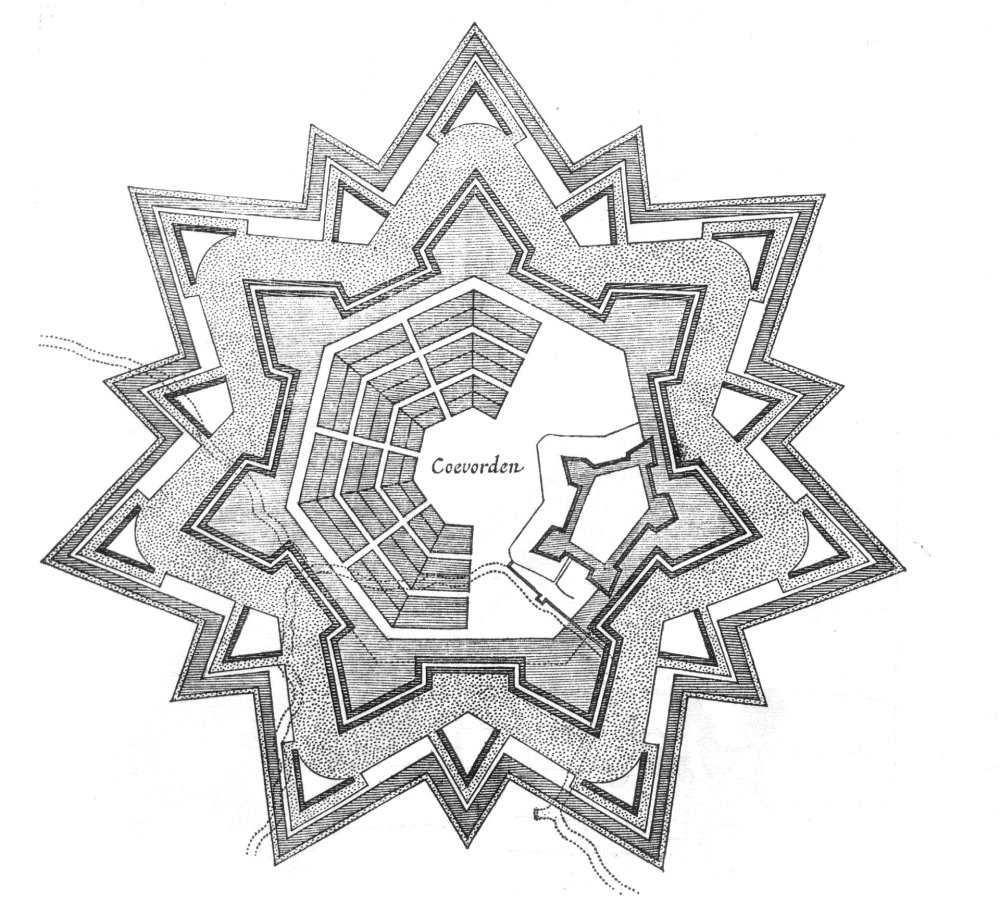
\includegraphics{Coevorden.jpg}
    \caption{Bastion fort}
    \label{bastion}
\end{marginfigure}
\marginpar{
    The bastion fort was a very flat structure composed of 
    many triangular bastions, specifically designed to cover each 
    other. To counteract cannonballs, defensive 
    walls were made stouter.
}

\subsection{The gunpowder revolution}
The gunpowder revolution lasted from the 1400s to the 1700s.
Prior to this, political power was decentralized amongst many 
of smaller powers. In Europe this manifested as hundreds of lords 
guided by the overarching influence of the Catholic church. Defense had the advantage. 
Sieges could last months or years, allowing the defenders an ever-present option to retreat. 
By and large, knights were the dominant power. The footmen were composed of untrained peasants 
forced into service by nobles. Between the 1400s and 1850 saw countries emerge from the 
disjoint political units, largely thanks to newly invented cannons capable of destroying castle walls. 
Defensive attempts to mitigate the destructive power of cannons, such as bastion forts, were expensive
and rare. Now that cannons were able to easily destroy castles, 
royalty needed a strong, constant military force to protect themselves. 
These trained armies were able to combat the poorly organized feudal knights 
and led to the solidification of nation states. Feudal states, independent cities, 
and religious enclaves had no ability to forward standing armies and were conquered 
and assimilated. No longer did skilled knights hold the advantage on the battlefield, 
but now masses of peasants taught to hold a gun straight and fire on command. 
Discipline became more important than skill. Lines of riflemen 
faced off on the battlefield, firing and firing again 
until enough musket balls had found their mark that the opposing line 
fell. 

As states with these larger armies assimilated their 
neighbors, Europe as we know it today began 
to emerge. Power solidified within families 
and individuals, and the medieval era of loose organization 
was supplanted by one of tighter regulation and control. 

\subsection{The Napoleonic revolution}
\subsection{The industrial revolution}
\subsection{The airpower revolution}
\subsection{The nuclear revolution}

\end{document}